\documentclass[11pt,a4paper]{article}

\usepackage[T1]{fontenc}
\usepackage[utf8]{inputenc}
\usepackage{lmodern}
\usepackage[margin=2.5cm]{geometry}
\usepackage{amsmath,amssymb}
\usepackage{graphicx}
\usepackage{booktabs}
\usepackage{caption}
\usepackage[section]{placeins}
\usepackage[numbers,sort&compress]{natbib}
\usepackage{xcolor}
\usepackage[colorlinks=true,linkcolor=blue!50!black,citecolor=blue!50!black,urlcolor=blue!50!black]{hyperref}

\captionsetup{font=small,labelfont=bf}
\graphicspath{{figures/}}
\newcommand{\T}{^{\top}}
\newcommand{\x}{\mathbf{x}}
\newcommand{\X}{\mathbf{X}}

\title{Do generated videos respect the geometry of a camera?\\[4pt]
\large Measuring AI-generated videos and images with the methods of the course}
% TODO: full names
\author{Khalil \and Ahmed\\[2pt]
\small CSC\_51073\_EP Image Analysis and Computer Vision, \'Ecole polytechnique}
\date{November 2026}

\begin{document}
\maketitle

\begin{abstract}
A real video is the output of a physical process: a rigid 3D scene, a camera that moves in
it, a lens, a sensor and a codec. A video generator only learns what such videos look like.
We ask whether this difference can be \emph{measured} with the classical tools of the course,
and we implement them ourselves in numpy: RANSAC, the normalized 8-point algorithm and the
Sampson distance (epipolar geometry between frames), linear triangulation and camera
calibration by DLT (a three-view test from the Structure-from-Motion lecture), vanishing
points by RANSAC on line segments (perspective), optical-flow warping (temporal coherence)
and the Fourier spectrum of the noise residual (upsampling traces). We run them on our own
paired clips (a real clip and generated clips started from its first frame) and on the
public ViF-Bench benchmark (165 real clips, 19 generators, 3160 videos). We add one method
from outside the course, a rigid-flow test that fits the instantaneous motion of a camera to
the optical flow given a learned depth map. Three findings stand out. (1) The raw epipolar
error mostly measures \emph{rendering}, not 3D: a control window copied from the real clip
shows the same gap. (2) The growth of the three-view reprojection error with the frame gap
separates geometry from blur on synthetic data, and it first seemed higher for generated
clips of ViF-Bench; once image motion and the noise floor of each clip are taken into account
the effect disappears (median ratio 1.004, $p=0.80$). At equal motion and equal precision we
do not detect a 3D drift on this benchmark. On our own scenes a difference appears only on
some scenes, and only relative to the real twin. (3) As a detector, our interpretable
features reach an AUC of 0.65 against 0.77 for a CLIP linear probe; they match CLIP on
image-to-video generators, and a late fusion of the two scores adds a small but significant
$+0.018$. We present the work as a set of measurements rather than as a detector, and we
provide a side-by-side demo that draws every method on the frames and ends with a
comparative verdict on the pair.
\end{abstract}

% ---------------------------------------------------------------------------
\section{Introduction}

Video generators such as Sora, Veo, Kling or Wan now produce clips that most viewers cannot
tell apart from camera footage. Detecting them matters for journalism, for legal evidence and
for the trust we put in any video shared online. The usual answer is a deep network trained
on real and generated examples. Such detectors work well on the generators they were trained
on, but recent benchmarks \cite{genvidbench,aigvdbench} show that they degrade on new
generators and after the recompression of social networks. They also do not say \emph{why}
a clip is suspicious.

We take the opposite angle. A real photo or video is the result of a physical chain:
3D scene $\rightarrow$ light $\rightarrow$ lens $\rightarrow$ sensor $\rightarrow$
processing $\rightarrow$ compression. Each link enforces constraints that a generator,
which learns the appearance of images and not the process behind them, has no reason to
satisfy exactly:
\begin{itemize}
  \item \textbf{multi-view geometry}: two frames of a static scene filmed by a moving camera
        satisfy $\x'^{\top}F\x=0$ for a single fundamental matrix $F$, and three frames are
        explained by one 3D point cloud and three cameras;
  \item \textbf{projective geometry}: parallel 3D lines meet at one vanishing point, and when
        the camera rotates all vanishing directions turn with the \emph{same} rotation;
  \item \textbf{temporal coherence}: once the motion is compensated, the texture of a real
        scene does not change from frame to frame, except for sensor noise;
  \item \textbf{signal processing}: camera noise has a smooth spectrum, while the upsampling
        layers of a generator leave periodic peaks \cite{durall2020,zhang2019}.
\end{itemize}

The goal of this project is to \emph{apply the methods of the course} to measure these
constraints, and to find out which measurements really see the 3D scene and which ones only
see the rendering. Building the best possible detector is not the goal; we compare with a
deep baseline only to place the measurements.

\paragraph{Contributions.}
\begin{enumerate}
  \item A numpy implementation of the core algorithms of Sessions 3, 4 and 7 (RANSAC, normalized
        8-point, DLT homography, Sampson distance, triangulation, camera DLT, vanishing points),
        validated against OpenCV and on synthetic scenes with known ground truth (89 unit tests).
  \item Four families of per-video measurements (V1 epipolar and three-view geometry,
        I2 vanishing points over time, V3 temporal coherence, I1 noise spectrum), computed by
        one reproducible pipeline (\texttt{python -m src.run}), and a fifth one from outside the
        course (V5, rigid flow with a learned depth map).
  \item Controls that tell geometry from rendering: a conditioning window copied from the
        real clip, synthetic clips that are blurred or slowly deformed, and comparisons at
        equal image motion.
  \item An evaluation on our own paired clips and on the full ViF-Bench benchmark, against a
        CLIP linear probe, per generator and with generators left out of training.
  \item A demo that plays a real clip and a generated clip side by side, draws every
        method on every frame with the values it computes, and ends with a comparative verdict
        (three-view error of the two clips at equal image motion, with a bootstrap interval).
\end{enumerate}

% ---------------------------------------------------------------------------
\section{Related work}

\paragraph{Frequency traces.}
Generators produce images at low resolution and upsample them, with transposed
convolutions in GANs or with the decoder of the variational autoencoder in latent diffusion
models. Zhang et al.\ \cite{zhang2019} showed that this upsampling leaves periodic peaks in
the Fourier spectrum of GAN images, and Durall et al.\ \cite{durall2020} that GANs fail to
reproduce the spectral distribution of real images at high frequency. Frank et al.\
\cite{frank2020} used the DCT spectrum as input of a simple classifier, and Corvi et al.\
\cite{corvi2023} found weaker but still visible peaks in the noise residual of diffusion
images. Our I1 module follows the same recipe with the filtering and Fourier tools of
Sessions 1--2: a noise residual, its log power spectrum averaged over frames, a radial
profile and a measure of periodic peaks.

\paragraph{Projective geometry.}
Sarkar et al.\ \cite{sarkar2024} (``Shadows don't lie and lines can't bend'') showed that
images from diffusion models often violate perspective: lines that should be parallel in 3D
do not meet at one vanishing point, and shadows are not consistent with one light source.
For videos, Grab-3D \cite{grab3d} uses the stability of vanishing directions over time in
static scenes. Our I2 module estimates vanishing points by RANSAC on LSD segments
\cite{lsd2010} and tests whether all vanishing directions move with one camera rotation.

\paragraph{Multi-view geometry.}
The fundamental matrix, the normalized 8-point algorithm \cite{hartley1997}, the Sampson
distance, triangulation and camera resectioning are classical
\cite{hartley2004}, and so is RANSAC \cite{fischler1981}. They are the subject of
Sessions 3, 4 and 7 of the course \cite{course}. Using them as a forensic test of a whole
video, rather than to reconstruct a scene, is the main idea of our V1 module. A full SfM
system such as COLMAP \cite{schoenberger2016} would be the natural next step.

\paragraph{Learned detectors and benchmarks.}
Ojha et al.\ \cite{ojha2023} showed that a linear probe on the features of a frozen CLIP
model \cite{radford2021} generalizes across image generators better than a network trained
end to end. We use this as our deep baseline (Session 5). For videos, GenVidBench
\cite{genvidbench} and AIGVDBench \cite{aigvdbench} show that detectors generalize poorly to
new generators. We evaluate on ViF-Bench \cite{vifbench}, which pairs each of 165 real clips
with the clips of 19 generators by file name, so that the content is matched.

\paragraph{Camera traces.}
Popescu and Farid \cite{popescu2005} detect the periodic correlations left by colour filter
array interpolation. These traces are destroyed by resizing and recompression; all public
video benchmarks are recompressed, so we did not pursue this bonus direction.

% ---------------------------------------------------------------------------
\section{Data and protocol}

\paragraph{Our paired clips.}
We filmed or selected real clips of static scenes with a moving camera (a field path, a
street at night, a rugby field, a city seen from a plane, a covered footbridge, a drone
rising above a suburb) and generated fake versions of the same scenes. Six generated clips
were made by image-to-video from the first frame of the real clip (Gemini Omni, Seedance~2
and other online generators whose name was not recorded), and two (\texttt{vid4fake},
\texttt{vid4fake2}) by \emph{video} continuation of the first 2~s of the real clip. This
gives 6 real and 8 generated clips in 6 paired scenes, plus 2 unpaired generated clips
(16 clips). Every file is listed in
\texttt{data/metadata.csv} with its generator, its conditioning (\texttt{cond\_type},
\texttt{cond\_s}) and its scene. Four more pairs (\texttt{vid7} to \texttt{vid10}) were added
at the end of the project and are used only in the demo (Section~\ref{sec:demo_res}); their
generators are not yet recorded in the metadata.

\paragraph{Normalization.}
Real and generated clips go through the same steps: 24~fps, short side 720~px (downscale
only, never upscale), H.264 with CRF~18, no audio. When reading the frames we drop the first
0.5~s (in image-to-video it is the real frame), keep at most 6~s, and crop the bottom 10\,\%
of every clip, real or generated, to remove visible watermarks. The demo can keep 1080~p
(\texttt{-{}-short-side 1080}) when both clips of a pair are 1080~p; pixel values at 1080~p are
not comparable with the 720~p values of the tables.

\paragraph{ViF-Bench.}
ViF-Bench \cite{vifbench} has 165 real clips and, for each, the clips of up to 19 generators
(open models such as Wan~2.1/2.2, HunyuanVideo, CogVideoX, LTX-Video, SkyReels, and closed
ones such as Sora~2, Kling, Hailuo, Pika, PixVerse, Gen-4). In total 3160 videos of about
5~s at 16~fps and 256~px height. Its parameters are in \texttt{configs/vifbench.yaml} (frame
gaps and thresholds scaled to the smaller frames). The full run took 26 minutes on a
16-core school machine. A scan of every frame of the benchmark
(\texttt{results/vifbench\_frame\_scan.csv}) shows three biases that matter for motion-based
measures: 5.5\,\% of the real clips are static, real clips contain irregularly duplicated
frames (variable frame rate), and 22\,\% of the CogVideoX clips are static. HunyuanVideo-I2V is
the only generator at 24~fps and $928\times544$~px; brought down to 256~px it is sharper than
the others.

\paragraph{Rules of comparison.}
Two rules come from our first experiments. First, generated clips often move less than real
ones, and every geometric error grows with image motion, so we compare real and generated
clips \emph{at equal image motion} (median flow of the pair), never at equal frame gap.
Second, a generated clip that received the first seconds of the real clip is a re-rendered
copy during that window; we compare only after the window and keep the window as a control.

% ---------------------------------------------------------------------------
\section{Methods}

All modules start with a header naming the course session they come from. The algorithms
of the course are our own numpy code (\texttt{src/geometry/}); OpenCV is used for SIFT, LSD,
Farneb\"ack flow and median filtering, and in the tests to check our implementations.

\subsection{Geometry core (Sessions 3 and 4)}

\paragraph{RANSAC.}
For a model with a minimal sample of $s$ points, an inlier ratio $w$ and a confidence $p$,
the number of rounds is $N=\log(1-p)/\log(1-w^{s})$; $N$ is updated each time a better
model is found, and the final model is refitted on all inliers (EP3, slides 100--112).

\paragraph{Fundamental matrix.}
With $\x=(u,v,1)^\top$ in image 1 and $\x'=(u',v',1)^\top$ in image 2, each match gives one
row of the linear system $A\mathbf{f}=0$:
\begin{equation}
  [\,u u',\; v u',\; u',\; u v',\; v v',\; v',\; u,\; v,\; 1\,]\;\mathbf{f}=0 .
\end{equation}
The solution is the right singular vector of $A$ with the smallest singular value, reshaped to
$3\times 3$; rank~2 is enforced by setting the smallest singular value of $F$ to zero. In the
normalized version \cite{hartley1997}, points are first mapped by similarities $T$, $T'$
(centroid at the origin, mean distance $\sqrt2$), and $F=T'^\top\hat F T$. RANSAC uses
$s=8$ and the Sampson distance
\begin{equation}
  d_S(\x,\x') = \frac{|\x'^\top F\x|}
  {\sqrt{(F\x)_1^2+(F\x)_2^2+(F^\top\x')_1^2+(F^\top\x')_2^2}},
\end{equation}
the first-order approximation of the geometric reprojection error \cite{hartley2004}, with
a threshold of 1.5~px on our clips (1.0~px on ViF-Bench).

\paragraph{Homography.}
The DLT gives two equations per match for the 9 entries of $H$; we use the same Hartley
normalization and a RANSAC with $s=4$ and the symmetric transfer error. In V1, $H$ tells
how much of the motion is explained by a plane or a pure rotation, a case where $F$ is
degenerate.

\paragraph{Vanishing points.}
A segment with end points $\mathbf{p}_1,\mathbf{p}_2$ gives the line
$\mathbf{l}=\mathbf{p}_1\times\mathbf{p}_2$; two lines give a candidate vanishing point
$\mathbf{v}=\mathbf{l}_1\times\mathbf{l}_2$ (EP4, slide 75). A segment is an inlier when the
angle between its direction and the line from its midpoint to $\mathbf{v}$ is below
$2^\circ$; this test also works for a point at infinity. The refit minimizes
$\sum_i(\mathbf{l}_i^\top\mathbf{v})^2$ with $\|\mathbf{v}\|=1$. Up to three vanishing
points are found by sequential RANSAC, removing the inliers of each one.

\subsection{V1: epipolar geometry between frames (Sessions 3 and 4)}

For pairs of frames $(t,t+\Delta)$ with $\Delta\in\{1,2,5,10,20,48,72,96\}$ frames, we detect
up to 4000 SIFT keypoints \cite{lowe2004} spread over an $8\times 8$ grid, match them with
the Lowe ratio test (0.75) and a mutual nearest-neighbour check, and estimate $F$ by RANSAC.
For each pair we record the share of matches that fit $F$, the median and 90th percentile
of the Sampson distance, the median image motion, and two context measures from the
homography: the share of $F$ inliers that $H$ also explains, and the \emph{parallax}, the
motion that $H$ cannot explain. Per video, the features are medians over pairs for each gap.

A pairwise test has a blind spot: $F$ only constrains a point to its epipolar line, so a
point that slides along this line (for example a depth that changes in time) is not seen.

\subsection{Three-view test (Session 7)}

The Structure-from-Motion lecture gives the tools to close this gap without the calibration
$K$. For a triplet of frames $(t,\,t+k,\,t+2k)$ with $k\in\{5,12,24\}$:
\begin{enumerate}
  \item Points are followed over the three frames by chaining the matches $t\to t+k$ and
        $t+k\to t+2k$.
  \item $F_{12}$ is estimated by RANSAC, and two projective cameras are built from it
        \cite[result 9.14]{hartley2004}:
        \begin{equation}
          P_1=[\,I\mid \mathbf{0}\,],\qquad P_2=[\,[\mathbf{e}']_\times F_{12}\mid \mathbf{e}'\,],
          \qquad F_{12}^\top\mathbf{e}'=0 .
        \end{equation}
  \item Each track is triangulated linearly: from $w\,\x=P\X$, each view gives
        $(\mathbf{p}^{3\top}\X)\,u-\mathbf{p}^{1\top}\X=0$ and
        $(\mathbf{p}^{3\top}\X)\,v-\mathbf{p}^{2\top}\X=0$; $\X$ is the singular vector of the
        $4\times4$ system with the smallest singular value.
  \item The camera $P_3$ of the third frame is estimated from the 3D--2D pairs by DLT
        (``camera calibration'' in the course: $A\,\mathrm{vec}(P_3)=0$, two equations per point,
        at least 6 points for the 11 degrees of freedom), inside RANSAC with a 2~px threshold.
  \item The reprojection error $\|\x_3-\pi(P_3\X)\|$ of the inliers is the measure.
\end{enumerate}
The reconstruction is only projective, which is enough for reprojection. Unlike the transfer
by intersection of epipolar lines, this test stays valid when the three camera centres are
aligned, which is the common case of a person walking straight ahead.

Because the error of every triplet depends on how precisely SIFT locates the points, which is
a rendering property, we use the \textbf{growth} of the median error with the gap,
\begin{equation}
  g = \frac{e_3(k_{\max})}{e_3(k_{\min})},
\end{equation}
as the geometric cue. A uniform loss of precision (blur, a different texture) scales both
errors and cancels in the ratio, while a scene that drifts slowly makes the error grow faster
with time.

\label{sec:methods_growth}The ratio only cancels a \emph{multiplicative} change. The error is closer to a sum
$e_3(k)\approx e_0+e_{\mathrm{geo}}(k)$ of a noise floor $e_0$ (point localization, which
depends on sharpness and compression) and a part that grows with the gap. Then
$g=(e_0+e_{\mathrm{geo}}(k_{\max}))/(e_0+e_{\mathrm{geo}}(k_{\min}))$: with the same geometry, a
sharper clip (lower $e_0$) has a larger $g$, and a clip that moves more has a larger
$e_{\mathrm{geo}}$ and a larger $g$. Two clips must therefore be compared at equal motion
\emph{and} equal floor; Section~\ref{sec:vif_growth} shows that this matters.

\subsection{I2: vanishing points over time (Sessions 1--4)}

On every second frame we detect LSD segments \cite{lsd2010} longer than 4\,\% of the image
diagonal and estimate up to three vanishing points. With an assumed camera
$K$ (focal length $0.8\times$ the longest side, principal point at the centre), each
vanishing point gives a 3D direction $\mathbf{d}=K^{-1}\mathbf{v}/\|K^{-1}\mathbf{v}\|$.
Directions are tracked from frame to frame (jump below $6^\circ$). In a rigid scene, when the
camera rotates by $R$ all directions turn together: $\mathbf{d}_i(t+1)\approx R\,\mathbf{d}_i(t)$.
We fit $R$ by orthogonal Procrustes on the tracked directions and record the angle left to
each direction (\emph{directions not explained by one rotation}), the variation of the angle
between two directions (a rotation keeps angles), and the misfit of the segments to their
vanishing point within one frame (a measure of how straight the rendered lines are).

\subsection{V3: temporal coherence by optical flow (Sessions 3 and 6)}

For pairs $(t,t+1)$ we compute the dense Farneb\"ack flow \cite{farneback2003} forward $f$ and
backward $b$. A pixel is kept when the forward-backward check
$\|f(\x)+b(\x+f(\x))\|<0.5+0.05\,\|f(\x)\|$ holds, which removes occlusions and flow failures.
Frame $t+1$ is warped back onto frame $t$ and we measure the residual on the kept pixels, on
its high-pass part divided by the noise level of the frame (fine texture that changes after
motion compensation, the ``boiling'' of generated videos), and on pixels that move less than
0.5~px. The share of pixels that fail the check is a feature too.

\subsection{I1: noise spectrum (Sessions 1 and 2)}

On 16 frames spread over the clip we compute the noise residual
$r=I-\mathrm{median}_{3\times3}(I)$, which removes the scene and keeps the noise, apply a Hann
window to the central square, and average the $\log_{10}$ power spectra
$\log_{10}|\mathcal{F}(r)|^2$. Averaging over frames lets periodic artifacts add up while the
random noise averages out. Features: the radial profile in 24 bins between 0 and
0.5~cycles/pixel, the slopes of the spectrum, the share of energy above 0.25~cycles/pixel, and
the \emph{periodic peaks}, the excess of each frequency over the mean of its ring (mean of the 8
strongest excesses).

\subsection{V5: rigid flow with a learned depth map (outside the course)}

The three-view test uses a few hundred SIFT points. V5 uses every textured pixel. For a camera
moving in a rigid scene, the instantaneous image motion of a pixel with normalized coordinates
$x=(u-c_x)/f$, $y=(v-c_y)/f$ and inverse depth $\rho=1/Z$ is \cite{longuet1980}
\begin{equation}
\begin{aligned}
\dot u &= \rho\,(-t_x + x\,t_z) + x y\,\omega_x - (1+x^2)\,\omega_y + y\,\omega_z,\\
\dot v &= \rho\,(-t_y + y\,t_z) + (1+y^2)\,\omega_x - x y\,\omega_y - x\,\omega_z ,
\end{aligned}
\end{equation}
with translation $\mathbf t$ and rotation rate $\boldsymbol\omega$. The translation part scales
with $\rho$ (parallax), the rotation part does not depend on depth. The inverse depth $d$ comes
from a monocular network, Depth Anything V2 small \cite{depthanything}, which is only defined up
to a scale and a shift: $\rho=a\,d+b$. Expanding, $\rho\,\mathbf t=d\,(a\mathbf t)+b\,\mathbf t$,
so the flow is \emph{linear} in nine unknowns $(a\mathbf t,\,b\mathbf t,\,\boldsymbol\omega)$.
We fit them by iteratively reweighted least squares (Cauchy weights) in numpy on the
Farneb\"ack flow over 8 frames, on textured pixels that pass the forward-backward check, with an
assumed focal length ($0.8\times$ the longest side). The per-pixel residual is the flow that no
camera motion explains given that depth: moving objects, or a generated scene whose motion
does not follow its own depth. Features: median residual, share of pixels above 1~px, and the
residual of a rotation-only model (what depth explains). Duplicated frames are skipped.
Code: \texttt{src/features/video\_rigidflow.py}; six tests check that an exact rigid flow is
recovered to $10^{-6}$~px, that the fit is invariant to the scale and shift of the depth, and
that a moving object stands out ($>2$~px) without disturbing the background ($<0.05$~px).

\subsection{Classification and baseline (Session 5)}

Each family gives a feature vector per video. We train a gradient boosting classifier (it
handles the missing values of clips without lines or without valid triplets) on each family
and on their union, and a logistic regression on the CLIP features. The CLIP baseline is a
linear probe on the mean ViT-B/32 embedding of 8 frames \cite{radford2021,ojha2023}. We use
5-fold cross-validation \emph{grouped by scene}, so a real clip and its generated versions are
always in the same fold and the classifier cannot match a fake to its twin. We report the
AUC with a bootstrap interval over scenes, the AUC per generator, and the AUC when the
tested generator is removed from the training folds (unseen generator).

\subsection{Demo}

\texttt{demo.py} measures every frame of a real and a generated clip with the functions above,
then writes a 1920$\times$1080 video and plays it in a window: the two clips side by side, one
method at a time drawn on the frames (points used in red, epipolar lines, three-view tracks
and their reprojection errors, segments coloured by vanishing point, the flow residual, the
noise spectrum), and a table of eleven values updated at every frame (Fig.~\ref{fig:demo}).

The last chapter gives a \emph{comparative} verdict (\texttt{src/demo/verdict.py}). Pixel
errors depend on the scene, the resolution and the motion, so a fixed threshold on one clip
would not mean much; the demo always has the real twin, so it compares the two. The judge is
the three-view reprojection error, chosen before looking at the pairs because it is the only
measure of the demo that tests one rigid 3D scene seen by one camera (the two-view inlier share
is a weak constraint, the Sampson distance mixes in the rendering, V3 and I1 measure the
signal). On the frames of both clips we fit
\begin{equation}
  \log e_3 = \alpha + \beta\,\log m + \gamma\,[\text{generated}],
\end{equation}
where $m$ is the image motion of the frame, so $\exp\gamma$ is the generated/real ratio at equal
motion. Its 95\,\% interval comes from a moving-block bootstrap of the frames (blocks of
0.5~s, since neighbouring frames are not independent). The verdict is ``the generated clip
agrees less with a real camera'' if the interval is above 1, ``the real clip agrees less'' if
it is below 1, ``no measurable difference'' otherwise, and no verdict when less than 30\,\% of
the frames lie in the motion range common to both clips (the fit would extrapolate). The
Sampson distance and the V3 texture change get the same fit and are shown as agreeing or not;
they do not change the verdict. Four unit tests check the four outcomes on synthetic series,
including that a clip that only moves more is not called less coherent.

% ---------------------------------------------------------------------------
\section{Results}

\subsection{Validation on synthetic data}

On a synthetic pair with known cameras, 200 matches, 30\,\% outliers and 0.5~px noise, our normalized
8-point RANSAC recovers $F$ with a median epipolar error of 0.14~px (Fig.~\ref{fig:synth},
left) and the sequential RANSAC separates the three families of a Manhattan box (right).
The tests check our $F$, $H$, triangulation, camera DLT and vanishing points against the
ground truth and against \texttt{cv2.findFundamentalMat} and \texttt{cv2.findHomography}.

\begin{figure}[!htbp]
  \centering
  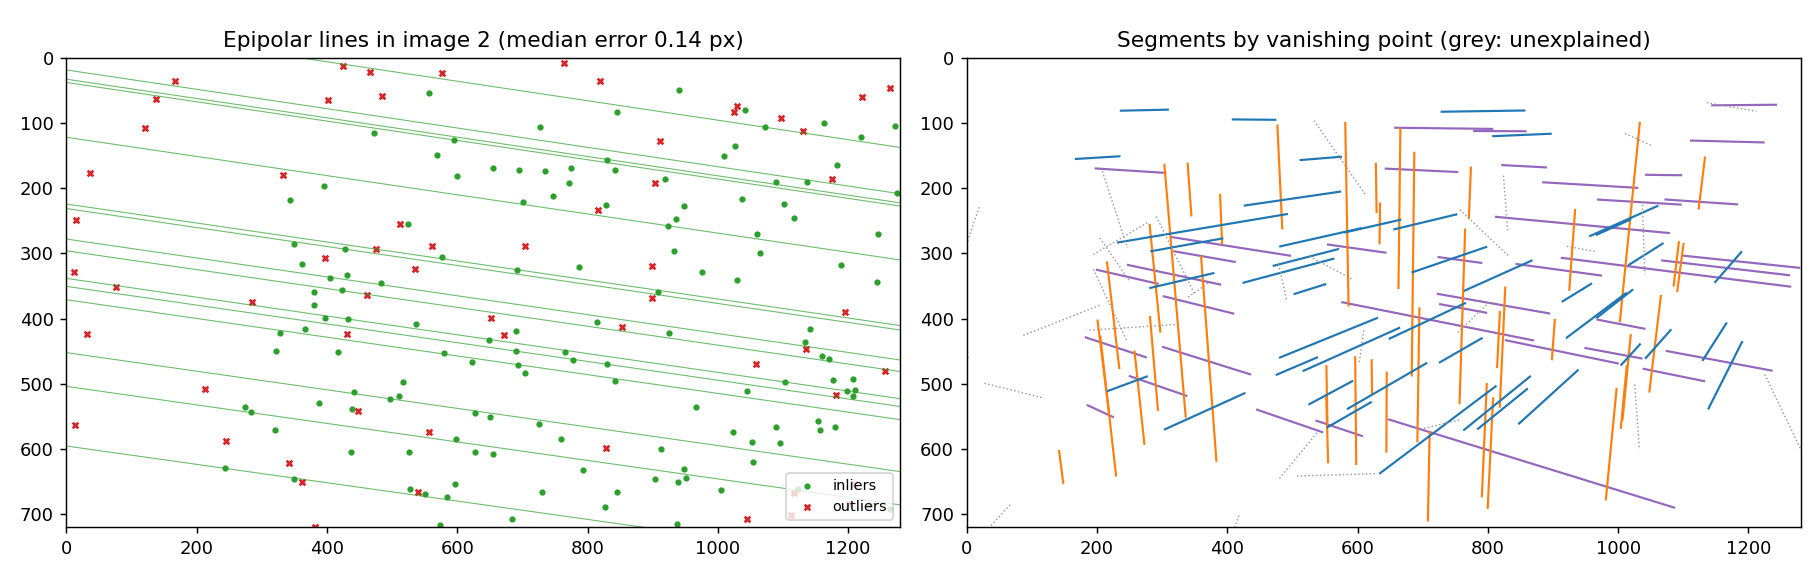
\includegraphics[width=\linewidth]{geometry_synthetic.png}
  \caption{Our implementations on synthetic data. Left: epipolar lines from our RANSAC +
  normalized 8-point estimate of $F$ (green inliers, red outliers). Right: segments grouped by
  our sequential RANSAC into three vanishing points (grey: no vanishing point).}
  \label{fig:synth}
\end{figure}

The more important question is \emph{what} each video measure reacts to. We rendered the same
rigid scene and camera path three times (\texttt{src/geometry/synth\_video.py}): clean,
blurred ($\sigma=1.5$~px, a pure rendering change), and slowly deformed (a 3D drift of up to
4~px). Table~\ref{tab:synth} shows the result. Blur raises the raw Sampson distance by 41\,\%
although the geometry is exact, so this measure is confounded with rendering. The growth of
the three-view error is unchanged by blur ($1.44\to1.41$) and more than doubles with the
drift ($1.44\to3.24$). V5 behaves the same way: its median residual at a gap of 8 frames is
0.385~px clean, 0.378~px blurred and 0.484~px with the drift ($+26\,\%$). On these clips the
camera path and the noise are the same for the three versions, so the growth is a fair
comparison; on real data it also depends on the noise floor and the motion
(Section~\ref{sec:vif_growth}).

\begin{table}[!htbp]
  \centering
  \begin{tabular}{lcc}
    \toprule
    Synthetic clip & Sampson median, gap 20 (px) & Three-view growth $g$ (gap 24 / gap 5) \\
    \midrule
    clean            & 0.090 & 1.44 \\
    blurred          & 0.127 (+41\,\%) & 1.41 \\
    slowly deformed  & 0.240 & 3.24 \\
    \bottomrule
  \end{tabular}
  \caption{What the V1 measures react to, on synthetic clips of one rigid scene
  (values from \texttt{tests/test\_synth\_measures.py}).}
  \label{tab:synth}
\end{table}

\subsection{The raw epipolar error measures rendering: the copied-window control}

On our first scene the generated clips were made by video continuation of the first 2~s of
the real clip. In the fakes, the first 2~s are a re-rendered copy of the real frames (PSNR
about 26~dB) and the generated content starts after. This window is a free control: real
geometry, generator rendering. At equal image motion, the median Sampson distance is
1.33 and 1.31 times higher on the two fakes than on the real clip over the whole clip, and
1.30 and 1.29 times higher \emph{inside the copied window}. The gap is the same where the
3D scene is the real one, so it comes from how the generator renders the frames (where SIFT
locates its points), not from a drifting scene. We had first presented the gap as a sign of
3D inconsistency; this control made us correct that claim. In the same window the three-view
growth is 0.99 and 0.91 times that of the real clip, as expected.

\subsection{Our paired scenes}

Table~\ref{tab:own} and Fig.~\ref{fig:growth_own} summarize the six scenes. The raw Sampson
ratio at equal motion goes both ways (0.67 to 1.70), which is consistent with a rendering
effect that depends on the generator and on the content. The three-view growth is equal for
three scenes (aerial city, footbridge with two generators) and lower for the field path,
where a person walks in the real clip and its grass moves in the wind. It is higher for the
rugby field, the night street and the drone scene.

\begin{table}[!htbp]
  \centering
  \small
  \begin{tabular}{llcccc}
    \toprule
    Scene & Clip & Sampson ratio & \multicolumn{2}{c}{Three-view error (px)} & Growth $g$ \\
          &      & gen./real$^\dagger$ & gap 5 & gap 24 & \\
    \midrule
    aerial city, night & real          & --   & 0.34 & 0.70 & 2.06 \\
                       & generated     & 0.67 & 0.21 & 0.43 & 2.07 \\
    field path         & real          & --   & 0.38 & 0.50 & 1.30 \\
                       & gen.\ 1 (2~s cond.) & 1.33 & 0.49 & 0.54 & 1.10 \\
                       & gen.\ 2 (2~s cond.) & 1.31 & 0.48 & 0.55 & 1.15 \\
    footbridge         & real          & --   & 0.64 & 1.09 & 1.70 \\
                       & Gemini Omni   & 1.70 & 0.64 & 1.09 & 1.70 \\
                       & Seedance 2    & 1.56 & 0.52 & 0.87 & 1.68 \\
    rugby field        & real          & --   & 0.94 & 0.88 & 0.94 \\
                       & generated     & 0.74 & 0.32 & 0.39 & 1.21 \\
    street, night      & real          & --   & 0.91 & 0.84$^*$ & 0.92 \\
                       & generated     & 1.52 & 0.88 & 0.90$^*$ & 1.03 \\
    suburb, drone rise & real          & --   & 0.29 & 0.47 & 1.62 \\
                       & generated     & 1.06 & 0.37 & 0.70 & 1.90 \\
    \bottomrule
  \end{tabular}
  \caption{V1 on our paired scenes (pipeline run on all 16 clips). $^\dagger$median Sampson
  distance at equal image motion, generated over real. $^*$gap 12: the night street clip is
  too short for gap 24. ``2~s cond.'': generated from the first 2~s of the real clip.}
  \label{tab:own}
\end{table}

\begin{figure}[!htbp]
  \centering
  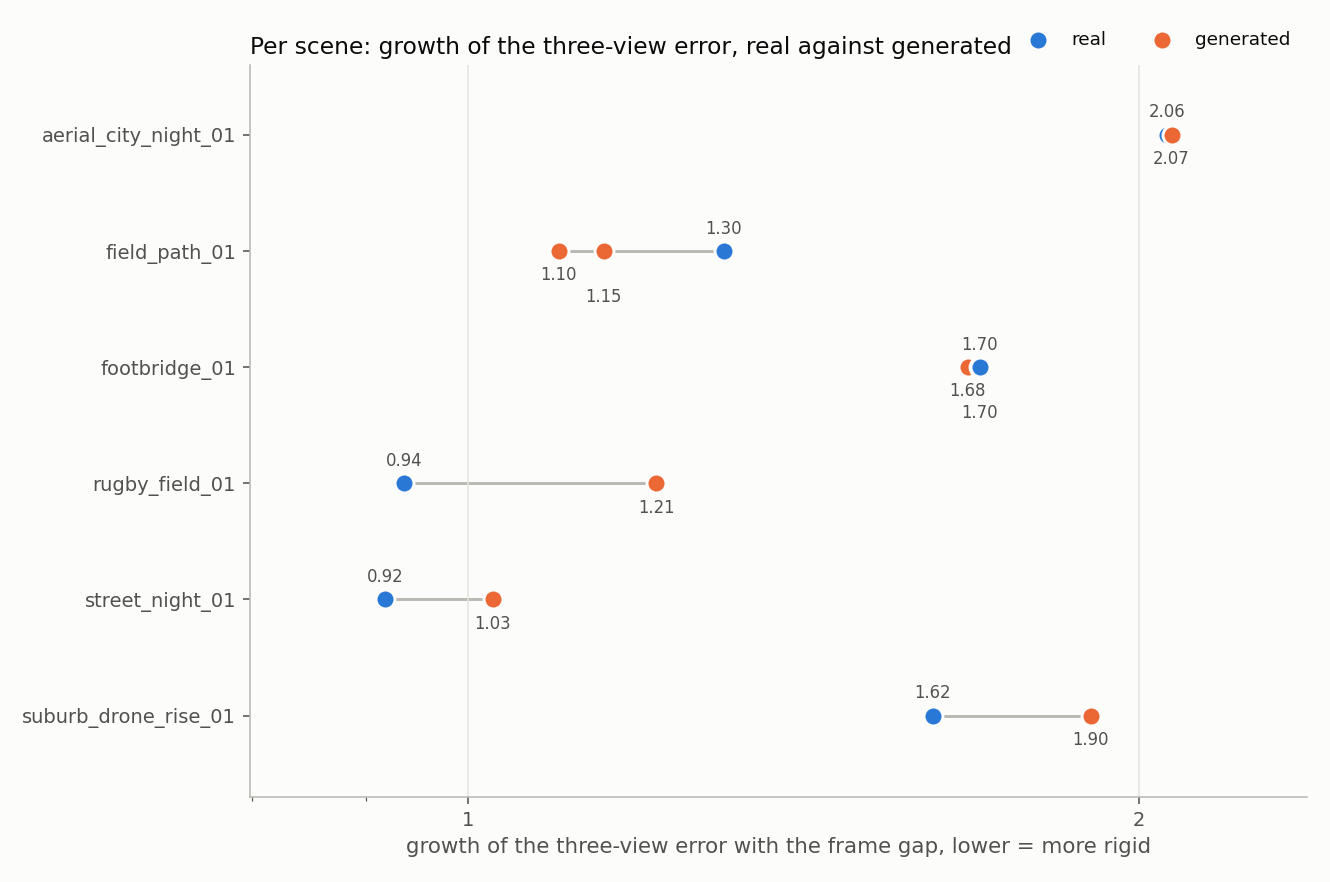
\includegraphics[width=0.8\linewidth]{v1_three_view_growth.png}
  \caption{Growth of the three-view reprojection error with the frame gap, per scene, real
  (blue) against generated (orange). Lower means a more rigid scene over time.}
  \label{fig:growth_own}
\end{figure}

\paragraph{When does a difference appear?}
The footbridge scene is the most favourable case for perspective (a steel frame, strong
Manhattan structure) but the camera only walks forward. Both generators keep its geometry:
equal growth, equal vanishing-point residuals. The drone scene is the opposite: the camera
starts at street level and rises above the houses, a large and smooth viewpoint change with
strong parallax (Fig.~\ref{fig:vid6}). It is the first scene where the generated clip has a
larger three-view error at every gap (+28 to +50\,\%) and a faster growth (1.90 against 1.62),
at similar image motion (5.3~px real, 6.0~px generated at gap 8). The I2 measures agree: the vanishing
directions of the generated clip are less well explained by one rotation
($0.98^\circ$ against $0.64^\circ$) and the angle between two directions varies more
($1.22^\circ$ against $0.49^\circ$); V3 sees pixels that do not move change more
(1.61 against 0.73 grey levels). Our reading is that generators keep the geometry of a
simple forward motion, which is close to what they see in training, and lose it when the
viewpoint changes a lot. Fig.~\ref{fig:vid6} (right) shows the I2 tracks of the generated
clip: direction 2 jumps by $13^\circ$ in 0.4~s and the angle between two directions moves by
$7^\circ$, which a rotating camera cannot do.

V5 agrees on the drone scene (Fig.~\ref{fig:v5}): the median residual of the rigid-flow fit is
0.57~px on the real clip and 0.97~px on the generated one, and 15\,\% against 48\,\% of the
pixels are more than 1~px away from the model. On the other scenes V5 has no constant
direction: on the footbridge the real clip has the larger residual (2.16~px against 1.08 and
0.81~px for the two generators), and on the rugby field it is far larger for the real clip
(6.65 against 0.11~px) because players move in it. V5 sees every non-rigid motion, moving
objects included, so it is only a geometric cue on scenes without moving objects.

\begin{figure}[!htbp]
  \centering
  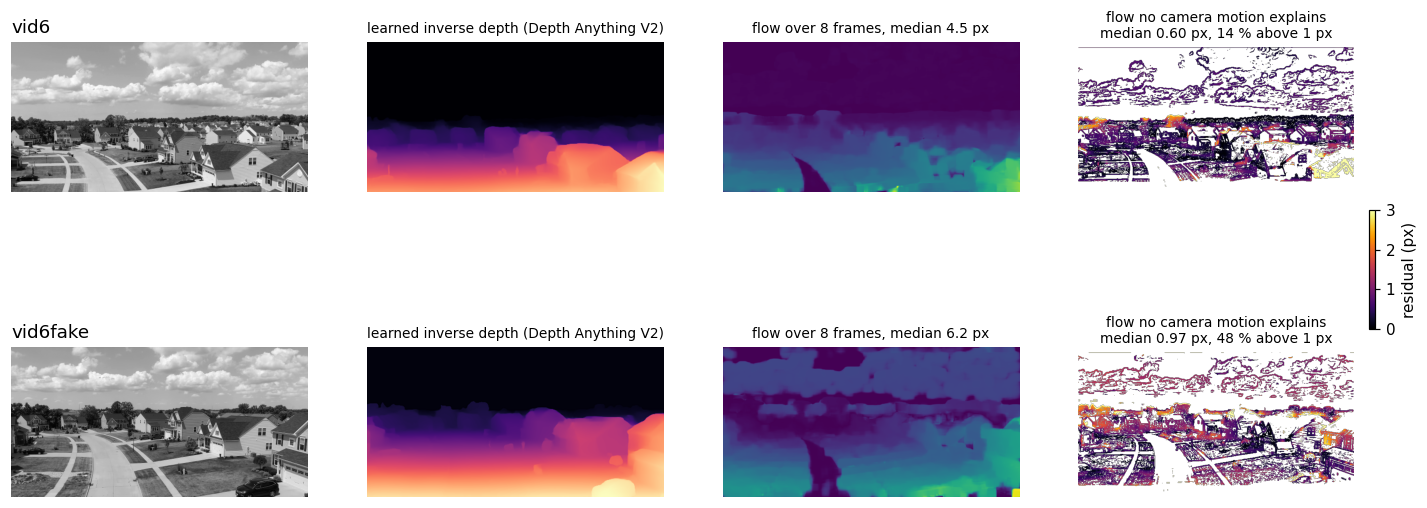
\includegraphics[width=\linewidth]{v5_residual_vid6.png}
  \caption{V5 on the drone scene, real (top) and generated (bottom): frame, learned inverse
  depth, flow over 8 frames, and the per-pixel flow that no camera motion explains given that
  depth.}
  \label{fig:v5}
\end{figure}

\begin{figure}[!htbp]
  \centering
  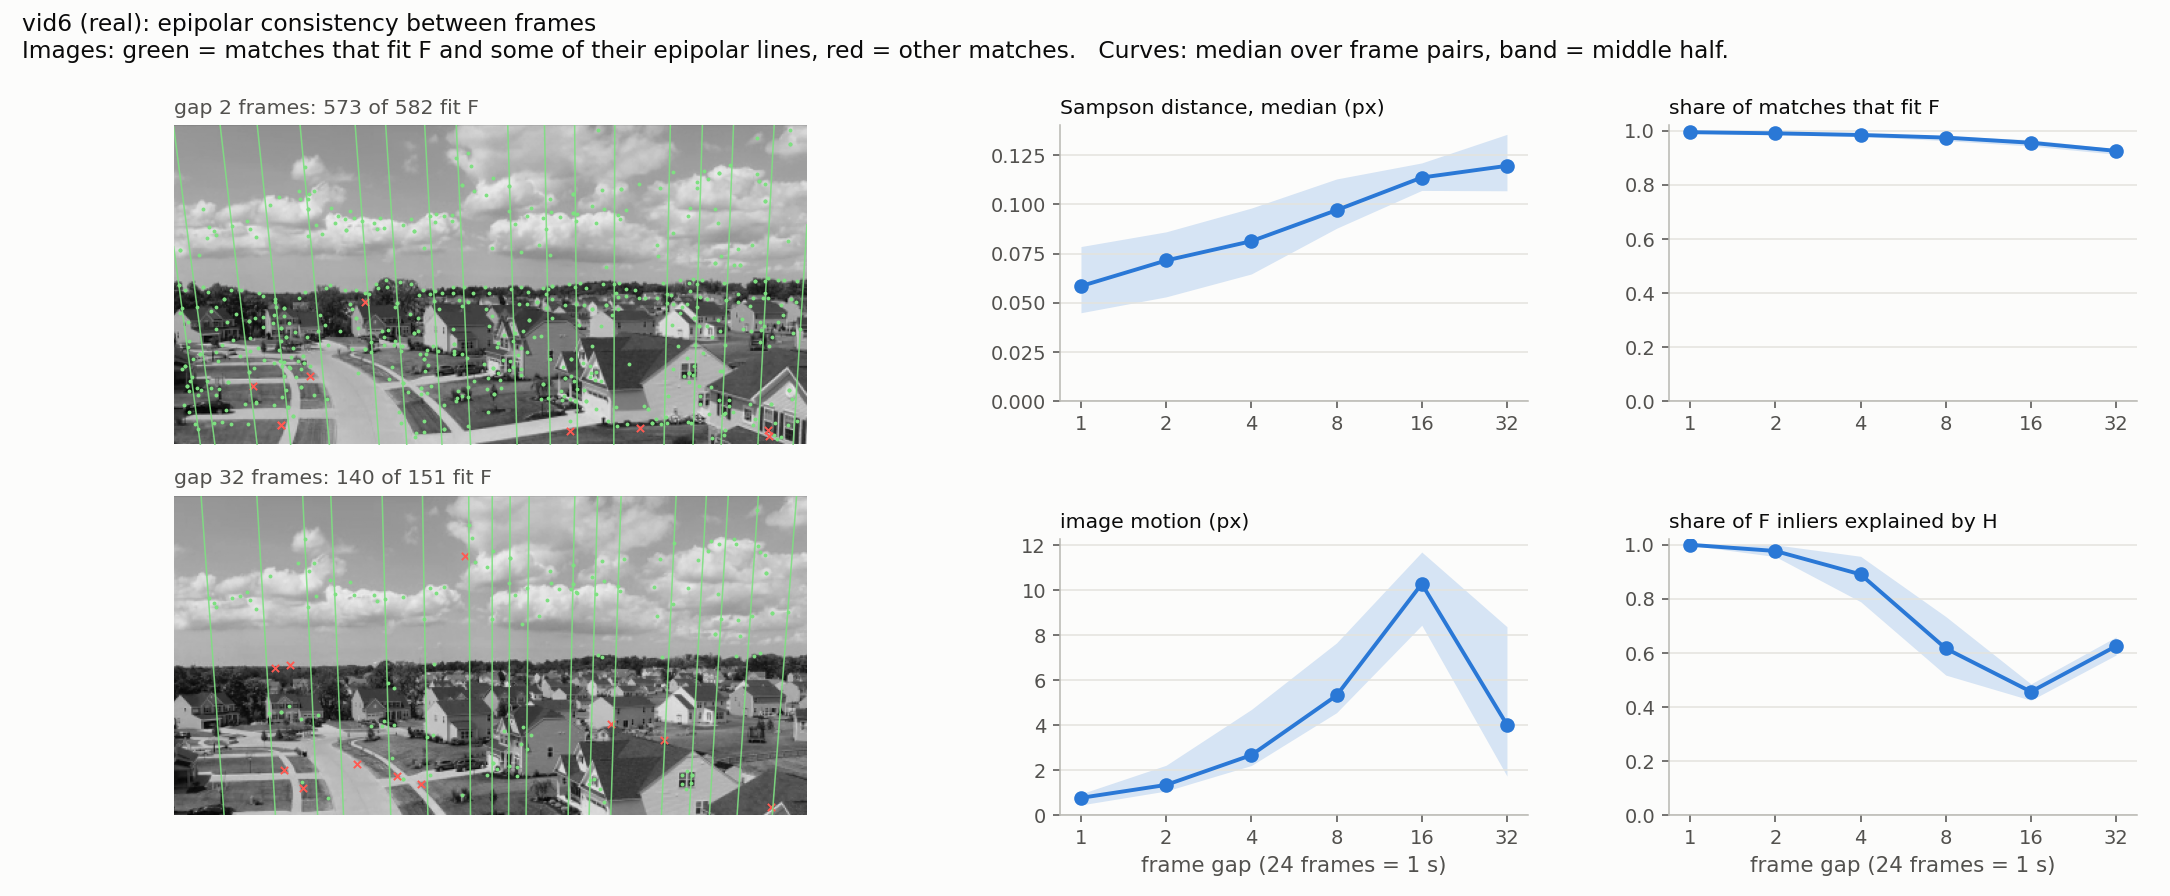
\includegraphics[width=\linewidth]{vid6_v1.png}\\[4pt]
  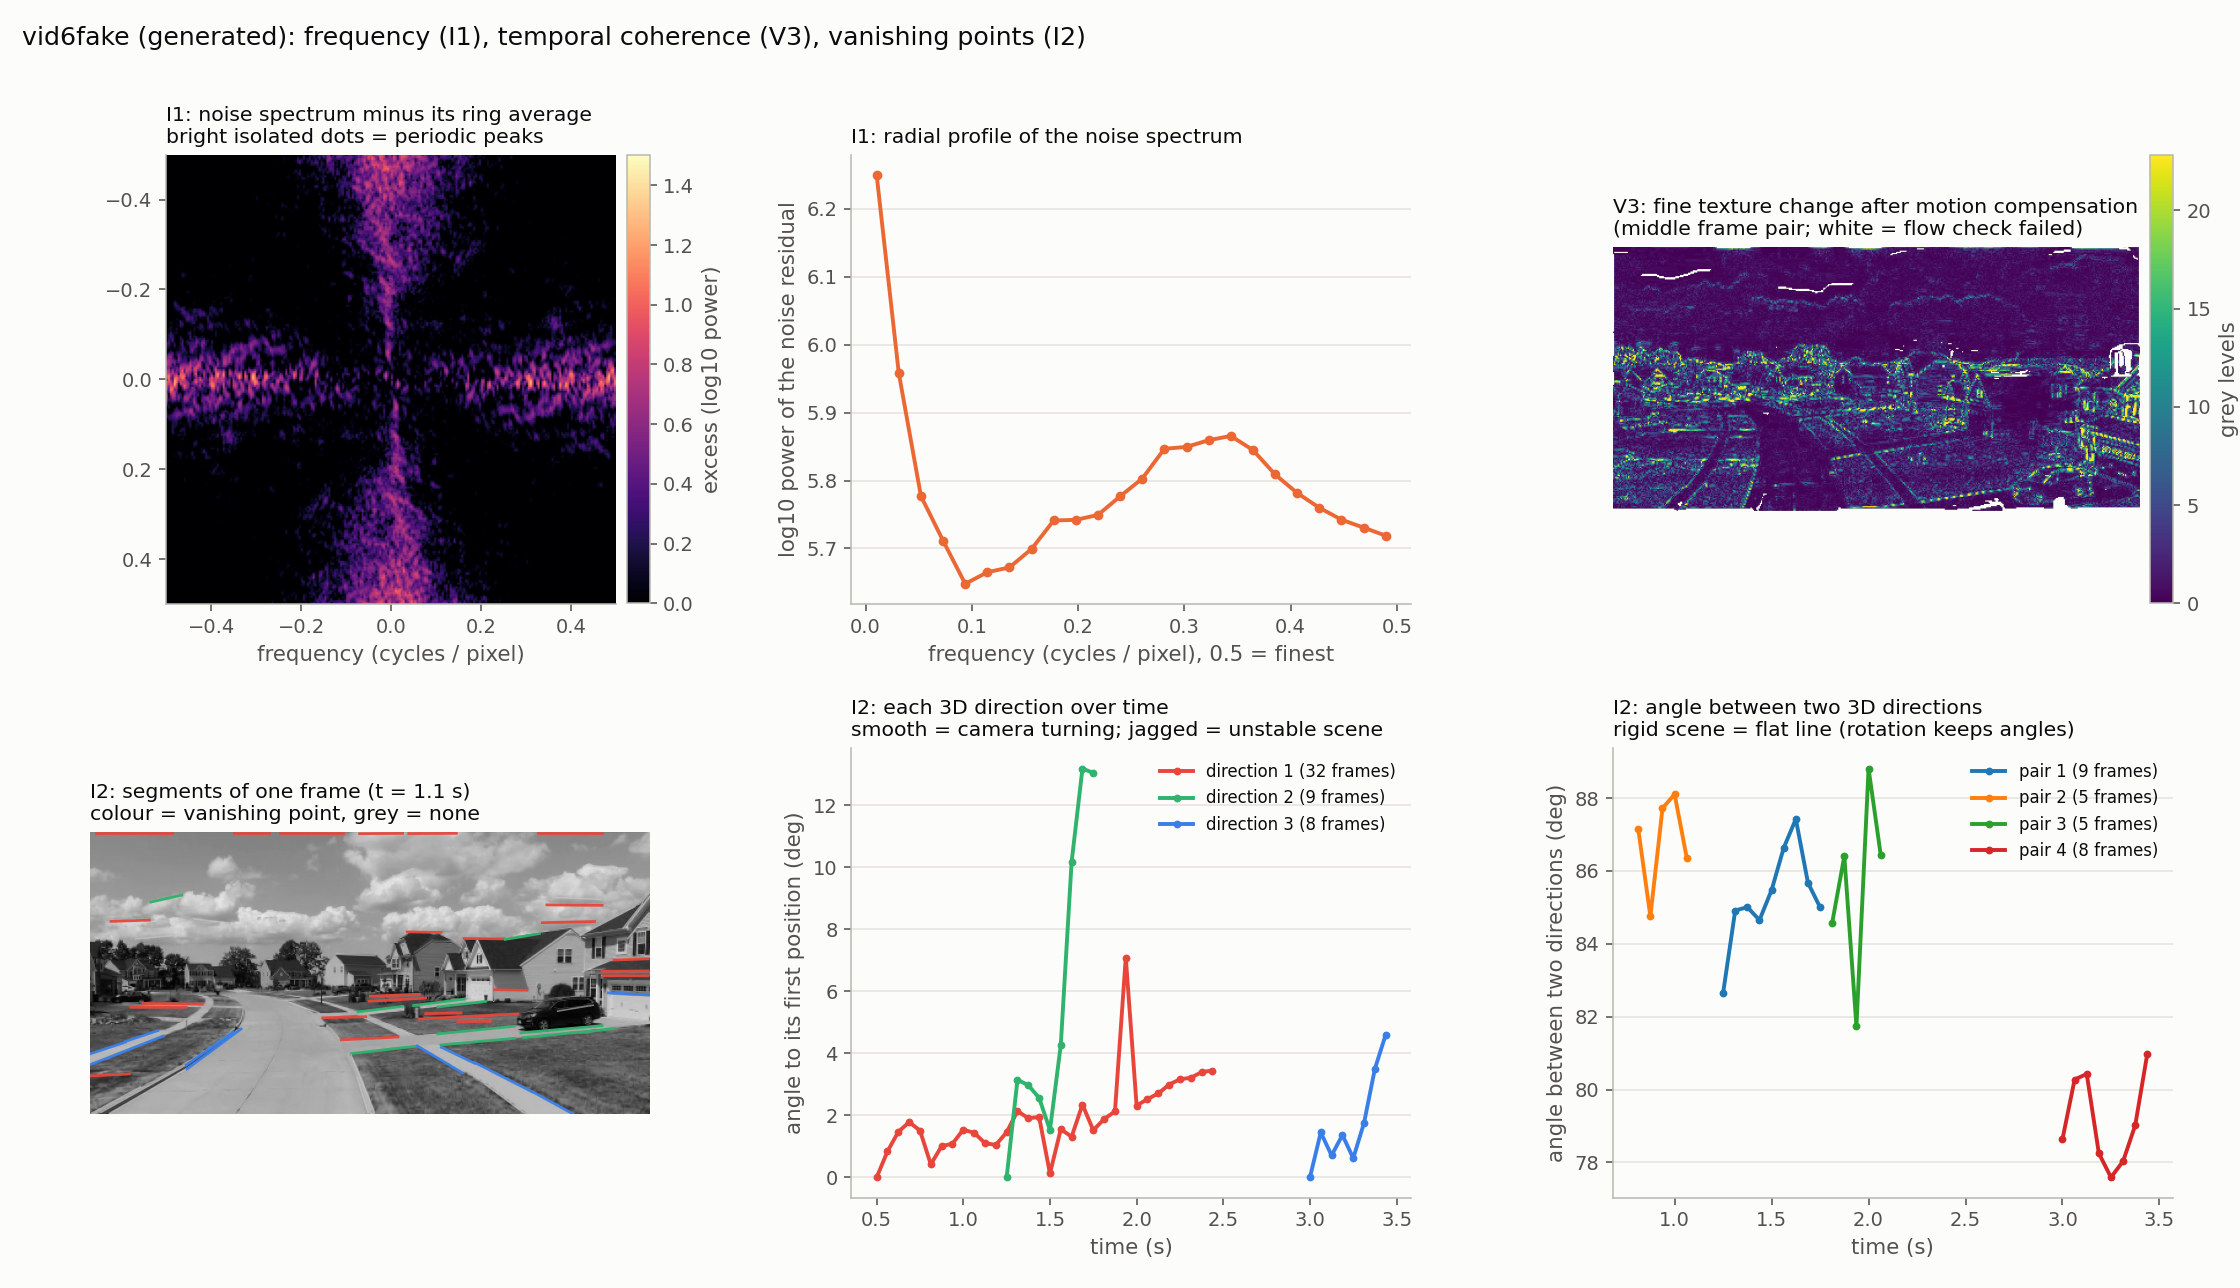
\includegraphics[width=\linewidth]{vid6fake_i1_v3_i2.png}
  \caption{Drone scene. Top: V1 on the real clip, matches that fit $F$ (green) with some
  epipolar lines; curves of the Sampson distance, inlier share, image motion and share
  explained by a homography against the frame gap. Bottom: the generated clip, I1 noise
  spectrum (excess over the ring average, radial profile), V3 texture change after motion
  compensation, and I2 (segments by vanishing point; 3D directions and angles between
  directions over time; a rigid scene gives smooth curves and flat angles).}
  \label{fig:vid6}
\end{figure}

\paragraph{Robustness on the drone scene.}
We re-encoded both clips at CRF~35 and halved their resolution, and re-measured them with the
inspection tool (ViF-Bench settings, gaps 3/8/16). The three-view error stays higher on the
generated clip: 0.29/0.36~px clean, 0.45/0.55~px at CRF~35, 0.23/0.32~px at half resolution.
The growth is higher on the generated clip clean (1.59 against 1.47) and at half resolution
(1.56 against 1.44) but not at CRF~35 (1.55 against 1.60). The difference survives these
degradations only partly, and it is visible only relative to the real twin: in absolute
terms both clips fall inside the range of real ViF-Bench clips.

\subsection{ViF-Bench: the three-view growth, and why it is not a 3D cue there}
\label{sec:vif_growth}

On ViF-Bench we compare each generated clip with the real clip of the same scene.

\paragraph{First reading.} Over all pairs the raw median growth ratio (generated / real) is
1.08, the generated clip has the larger growth in 58\,\% of the pairs (Wilcoxon test over
scenes, $p=0.002$), and the growth alone gives an AUC of 0.58. The raw ratio depends on the
generator (Fig.~\ref{fig:growth_vif}): it is highest for HunyuanVideo-I2V (1.30), LTX-Video-13B
text-to-video (1.29) and Sora~2 (1.18), and below 1 for Wan~2.2, HunyuanVideo, Pika and
CogVideoX (0.94 to 0.97). The raw Sampson ratio goes from 0.73 (LTX-Video) to 1.26 (CogVideoX):
it changes sign across generators, as expected from a rendering effect.

\paragraph{Check against the noise floor and the motion.} Section~\ref{sec:methods_growth}
showed that the growth rises when the noise floor falls or the motion rises, with the same
geometry. Both differ between real and generated clips on ViF-Bench. The growth ratio of a pair
follows the ratio of the noise floors (three-view error at the smallest gap; Spearman $-0.21$,
$p=10^{-25}$), and across generators it follows the ratio of image motions ($-0.56$, $p=0.01$).
HunyuanVideo-I2V, the generator with the largest ratio, is the only one at $928\times544$~px
and 24~fps: brought down to 256~px it is sharper than the others, so its floor is lower and its
growth higher. Once these two effects are removed the difference is gone:
\begin{itemize}
  \item on the 353 pairs whose image motions are comparable, the median growth ratio is 1.002
        ($p=0.61$);
  \item after regressing the log growth ratio on the log motion ratio and the log floor ratio,
        the median residual ratio is 1.004 (Wilcoxon $p=0.80$).
\end{itemize}
At equal motion and equal precision, we do not detect a 3D drift of the generated clips of
ViF-Bench. The first reading measured how much and how sharply the clips move, not their
geometry. This is the main correction of this report: an earlier version presented the raw
per-generator ratios as a geometric effect.

\begin{figure}[!htbp]
  \centering
  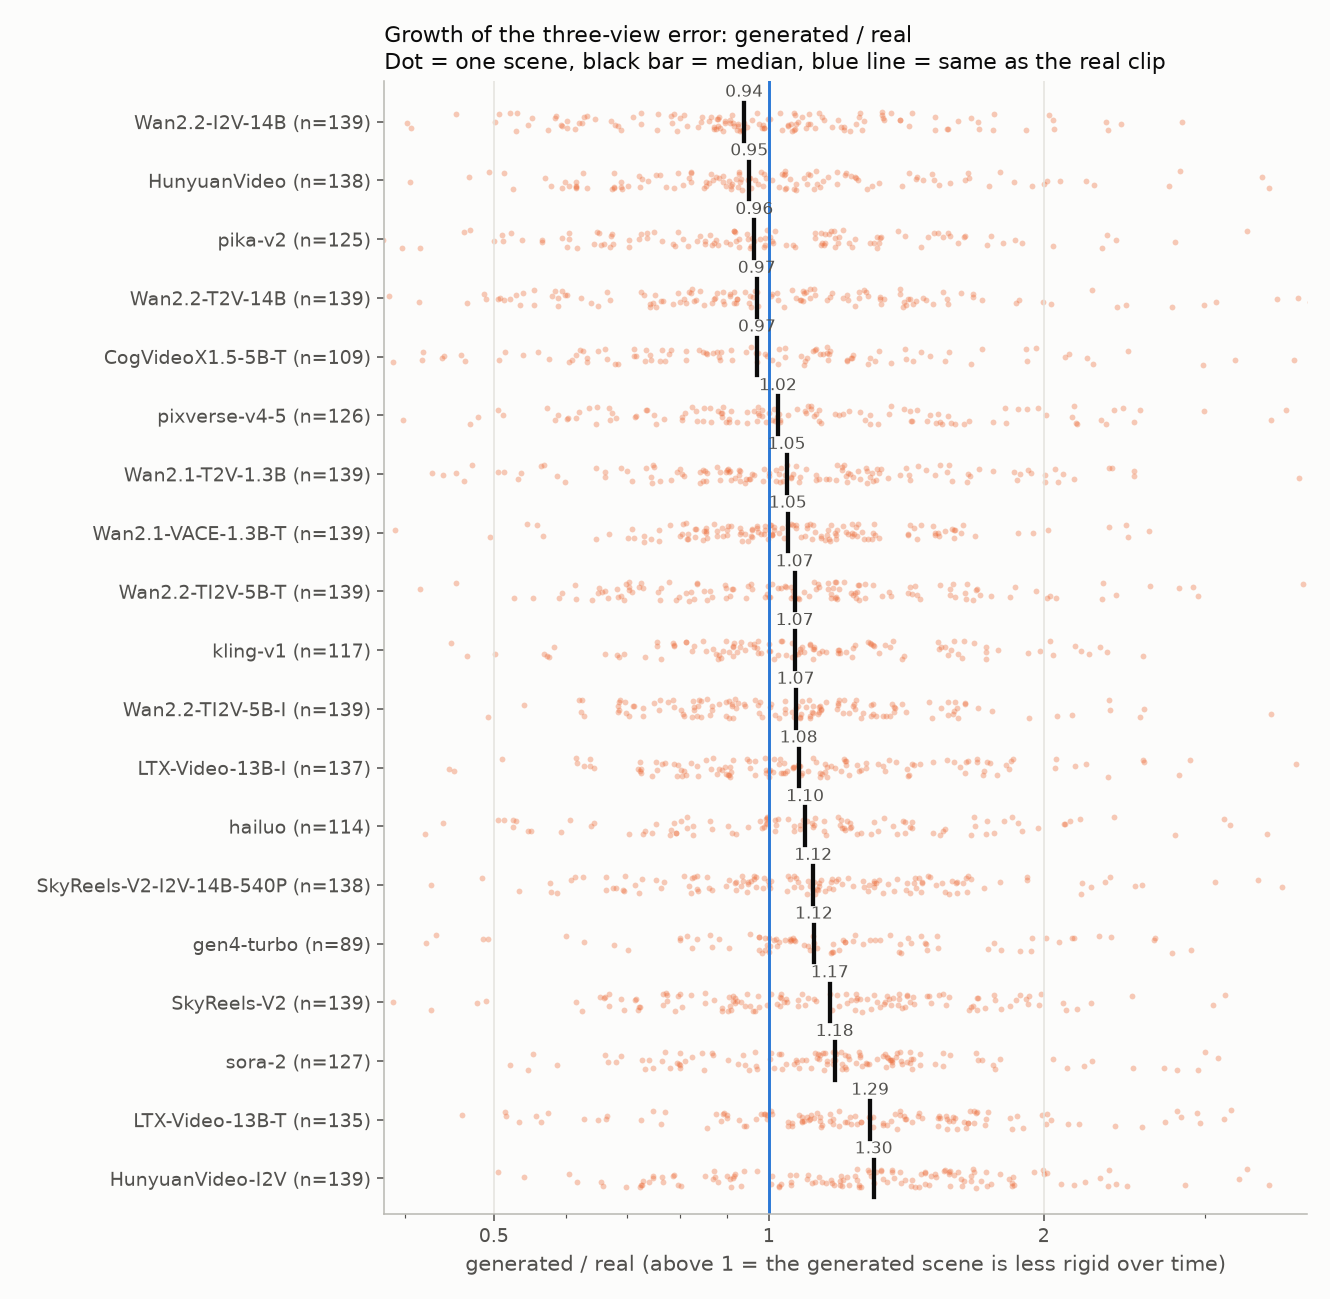
\includegraphics[width=0.78\linewidth]{v1_growth_ratio_by_generator.png}
  \caption{ViF-Bench: \emph{raw} growth of the three-view error, generated over real, one dot per
  scene, black bar = median. These ratios are not corrected for motion and noise floor; after
  correction the pooled median is 1.004 (Section~\ref{sec:vif_growth}).}
  \label{fig:growth_vif}
\end{figure}

\subsection{ViF-Bench: classification}

Table~\ref{tab:clf} gives the cross-validated results. V1 geometry alone reaches an AUC of
0.62 and I1 frequency 0.56. The V3 row (0.49) is not a measurement of temporal coherence: on
these small and recompressed frames most of the V3 per-video features were medians of
quantities that are zero on most pixels (residual and flow of still pixels), so the features
were degenerate; they were also computed with an earlier version of the code. A corrected
prototype (textured pixels only, means instead of medians, duplicated frames skipped) is still
at chance pooled over generators (AUC 0.5), and its per-generator ratios go both ways, like a
rendering signature. The union of our features reaches 0.65 and the CLIP linear probe 0.77.
Concatenating our features with CLIP in one classifier does not improve CLIP, because the 512
CLIP dimensions dominate. A late fusion does: averaging the ranks of the two scores (weight
0.25 for the physics score) gives 0.786, a gain of $+0.018$ over CLIP (interval
$[0.008, 0.030]$, 500 bootstraps over scenes). The weight was chosen on the same data, so the
gain is slightly optimistic; with a weight of 0.35 it is $+0.017$ $[0.001, 0.033]$. Our
features therefore carry a little information that CLIP does not. The balanced accuracy of the physics
classifiers stays near 0.52 because the classes are unbalanced (165 real for 2995
generated) and the default threshold predicts almost always ``generated''; the AUC is the
meaningful number here.

\begin{table}[!htbp]
  \centering
  \small
  \begin{tabular}{lrccc}
    \toprule
    Features & dim. & AUC [95\,\% interval] & AUC, mean over & AUC, mean over \\
             &      &                       & generators & unseen generators \\
    \midrule
    V1 geometry (Sessions 3, 4, 7)   & 77  & 0.62 [0.58, 0.67] & 0.62 & 0.60 \\
    I1 frequency (Sessions 1--2)     & 30  & 0.56 [0.52, 0.60] & 0.56 & 0.54 \\
    V3 temporal (Session 6)$^*$      & 8   & 0.49 [0.44, 0.54] & 0.49 & 0.46 \\
    physics (V1 + I1 + V3)           & 115 & 0.65 [0.61, 0.69] & 0.65 & 0.62 \\
    CLIP linear probe (Session 5)    & 512 & 0.77 [0.74, 0.80] & 0.77 & 0.75 \\
    physics + CLIP, concatenated     & 627 & 0.77 [0.74, 0.79] & 0.77 & 0.74 \\
    physics + CLIP, late fusion      & --  & 0.786             & --   & --   \\
    \bottomrule
  \end{tabular}
  \caption{ViF-Bench, 3160 videos, 5-fold cross-validation grouped by scene. Last column:
  each generator is removed from training and then tested. $^*$Degenerate features (see text).
  Late fusion: rank average of the physics and CLIP scores, gain over CLIP $+0.018$
  $[0.008, 0.030]$. I2 and V5 were not run on the full benchmark.}
  \label{tab:clf}
\end{table}

\paragraph{Per generator and per kind of conditioning.}
Fig.~\ref{fig:pergen} breaks the AUC down by generator. Our features beat CLIP only for
HunyuanVideo-I2V (0.73 against 0.67) and Gen-4 Turbo (0.65 against 0.65), and are close for
the other image-to-video generators. Grouping the generators by conditioning makes this
clear: on image-to-video generators our features and CLIP are equivalent (AUC 0.65 against
0.66, difference 0.01 with interval $[-0.04, 0.06]$), while on text-to-video generators CLIP
wins by 0.15. A text-to-video clip has different content and style from its real
counterpart, which CLIP sees at once; an image-to-video clip starts from the real frame, so
only its evolution can differ, and that is what our geometric measures look at.

\paragraph{Camera motion or 3D coherence?}
Part of what V1 detects is simply that generated clips move differently: a classifier on the
camera-motion features alone (image motion, parallax, share explained by a homography)
reaches an AUC of 0.59. Adding the coherence features on top of motion and matching features
gives no gain over all generators ($-0.0005$), but a gain of $+0.044$ (interval
$[0.010, 0.078]$) on image-to-video generators. The coherence features corrected for motion
reach 0.62 alone. Given Section~\ref{sec:vif_growth}, we read this gain with care: the
coherence features are corrected for motion but not for the noise floor, so part of it may
still come from how sharply the clips are rendered rather than from their 3D geometry.

\begin{figure}[!htbp]
  \centering
  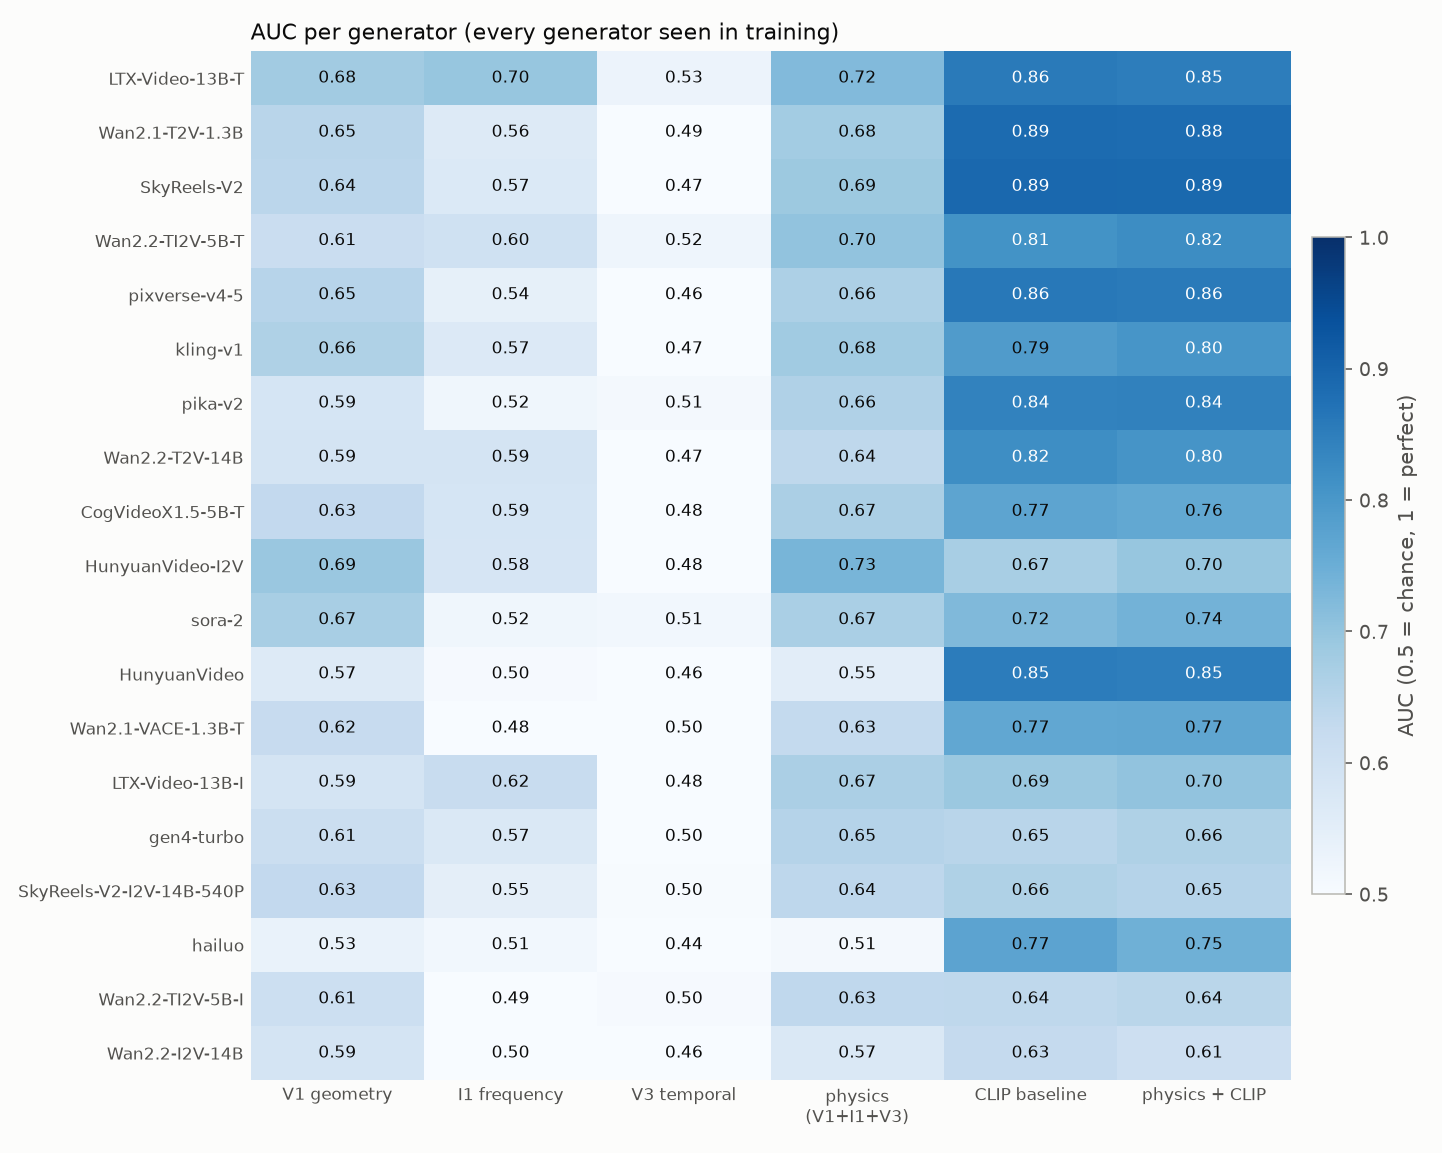
\includegraphics[width=0.85\linewidth]{classify_per_generator.png}
  \caption{ViF-Bench: AUC per generator (all real clips against the clips of that generator),
  for each family of features and for the CLIP baseline.}
  \label{fig:pergen}
\end{figure}

\subsection{The demo}
\label{sec:demo_res}

The demo (Fig.~\ref{fig:demo}) is the result of running \texttt{demo.py} on the drone scene.
All values come from our code, computed on each frame: about 1~s per frame and per clip on
CPU, so the frames are computed first (in parallel, about 3 minutes for two 6~s clips, then
cached) and the video is played afterwards. The values in the table are running medians over
the frames seen so far; at the end they match the pipeline values (three-view error 0.37
against 0.51~px, the pipeline gives 0.38 against 0.49~px). The I2 rotation residual of the demo
differs from the pipeline (0.99 against 0.97 instead of 0.59 against 0.62), probably because
the demo uses the whole clip and a different random draw per frame; we did not verify this.
LSD also sometimes detects the top border of the frame as a segment (the yellow line at the
top of Fig.~\ref{fig:demo}, right).

\begin{figure}[!htbp]
  \centering
  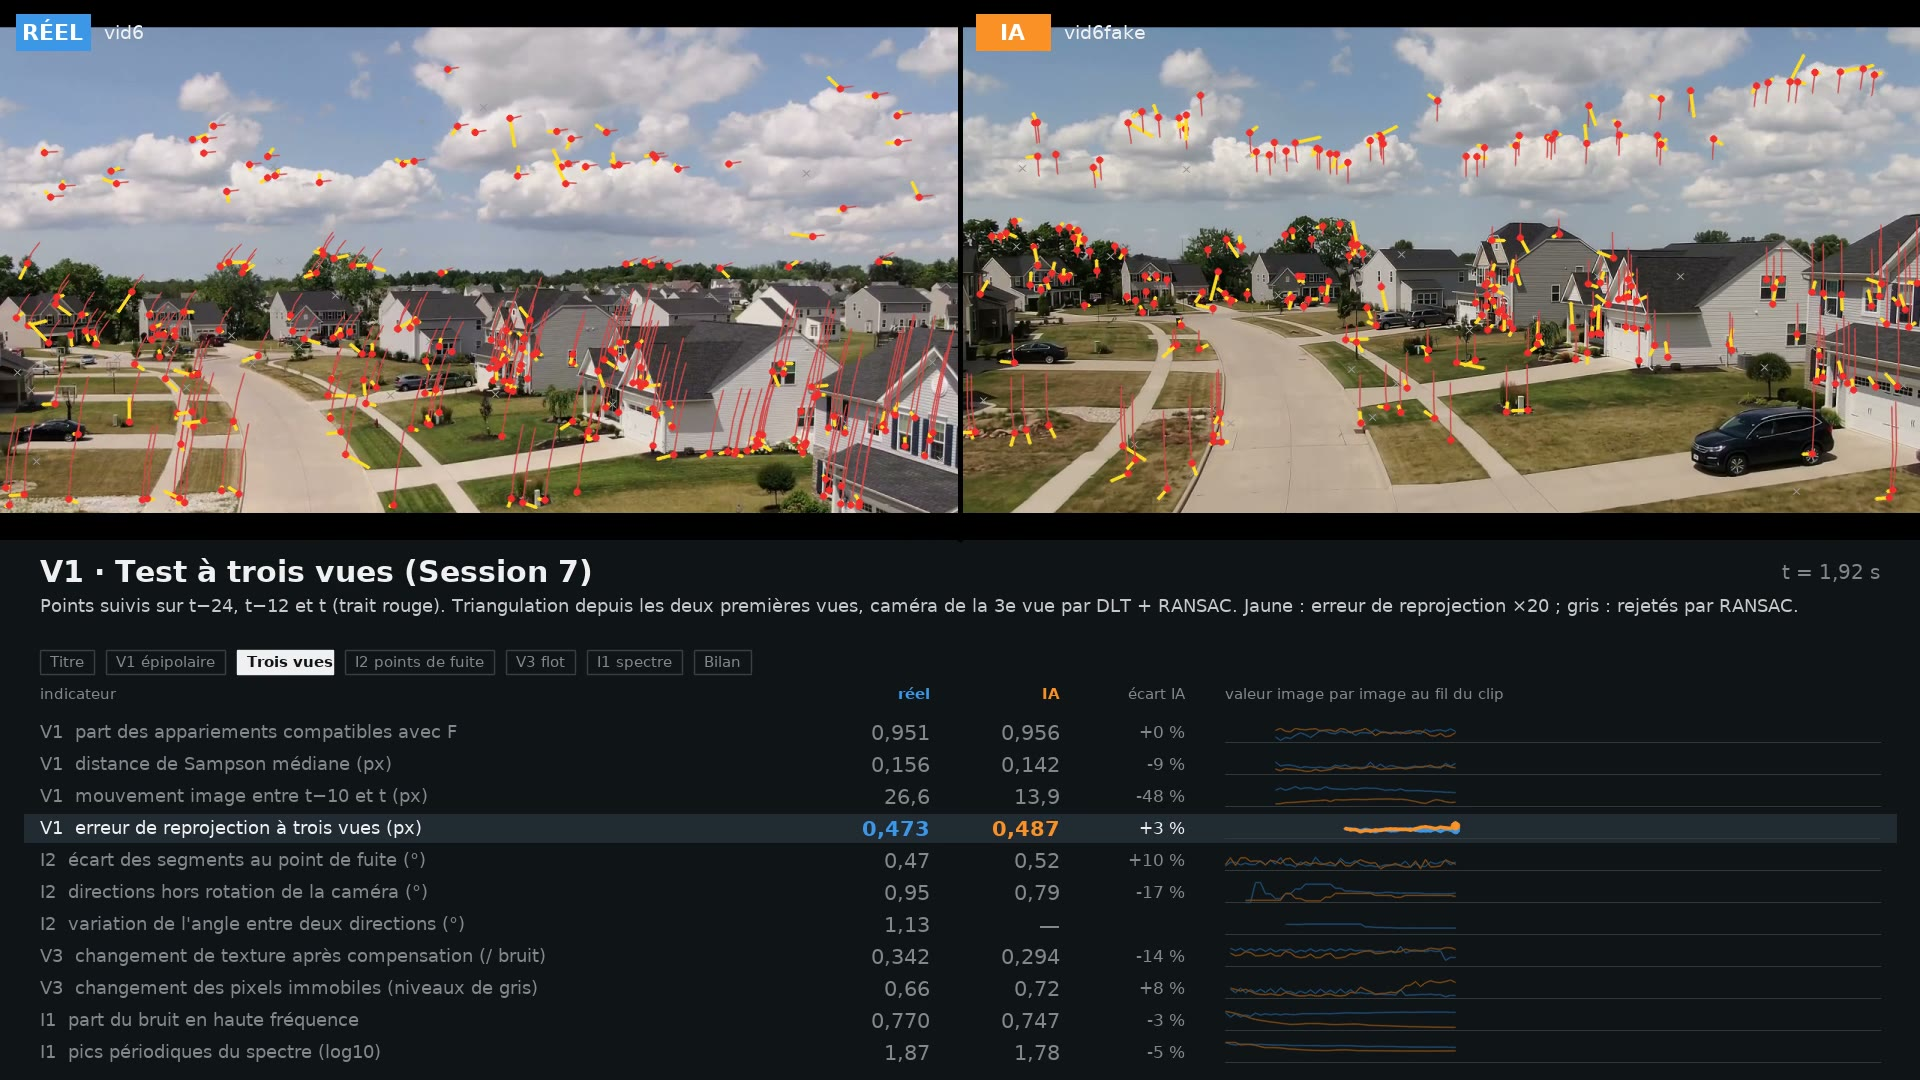
\includegraphics[width=0.49\linewidth]{demo_three_view.jpg}\hfill
  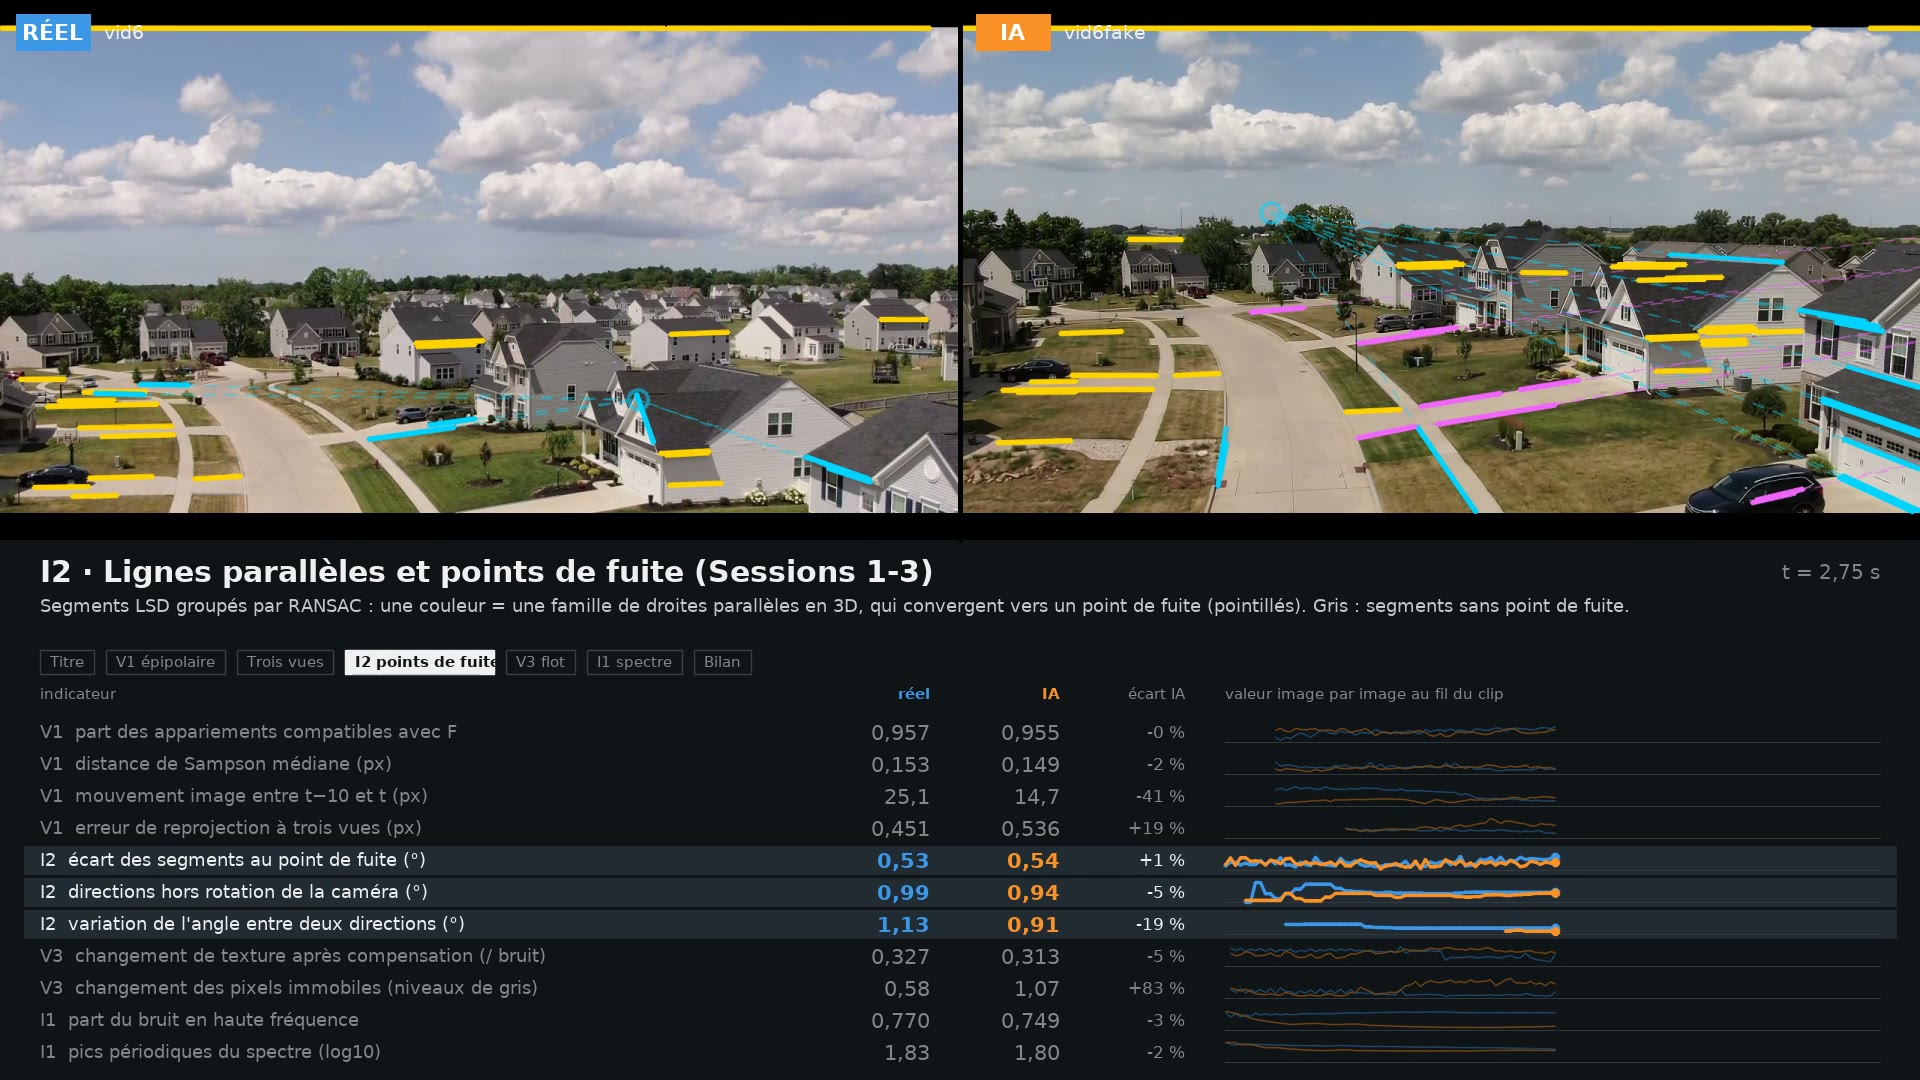
\includegraphics[width=0.49\linewidth]{demo_i2.jpg}
  \caption{Two frames of the demo on the drone scene (real left, generated right in each
  frame). Left: three-view test, tracks over $t-24$, $t-12$, $t$ in red, reprojection error
  in yellow (magnified 20 times), RANSAC outliers in grey. Right: segments coloured by
  vanishing point, dashed lines toward the vanishing point. Below the frames, the table of
  values updated at every frame, with their curves over the clip.}
  \label{fig:demo}
\end{figure}

\paragraph{Verdict on six pairs.} Table~\ref{tab:verdict} gives the verdict of the demo on the
pairs \texttt{vid5} to \texttt{vid10} (1080~p when both clips are 1080~p, 720~p otherwise).
The generated clip is called less coherent on two pairs (drone scene, \texttt{vid9}), with the
Sampson distance agreeing; the real clip is called less coherent on \texttt{vid8}; there is no
measurable difference on \texttt{vid10}, and no verdict on two pairs whose camera motions do
not overlap (\texttt{vid5}: 1\,\% of the frames in the common range). Six pairs are an
illustration, not an evaluation: the verdict compares two clips of one scene and is not a
detector. Choosing and weighting the measures on ViF-Bench and testing them blind on our pairs
is the next step.

\begin{table}[!htbp]
  \centering
  \small
  \begin{tabular}{lcccl}
    \toprule
    Pair & Res. & Three-view error, gen./real & Motion & Verdict \\
         &      & at equal motion [95\,\%]   & overlap &         \\
    \midrule
    \texttt{vid5} (footbridge)             & 720~p  & 0.95 [0.72, 1.17] & 1\,\%  & no verdict \\
    \texttt{vid6} (drone)                  & 1080~p & 1.54 [1.42, 1.65] & 85\,\% & generated less coherent \\
    \texttt{vid7}                          & 720~p  & 1.17 [1.08, 1.38] & 20\,\% & no verdict \\
    \texttt{vid8}                          & 1080~p & 0.86 [0.73, 0.93] & 62\,\% & real less coherent \\
    \texttt{vid9}                          & 1080~p & 1.80 [1.35, 2.21] & 69\,\% & generated less coherent \\
    \texttt{vid10}                         & 1080~p & 1.29 [0.88, 1.59] & 78\,\% & no difference \\
    \bottomrule
  \end{tabular}
  \caption{Comparative verdict of the demo (\texttt{python demo.py REAL FAKE -{}-no-video}).
  Motion overlap: share of the frames of both clips inside the motion range common to the two;
  below 30\,\% the demo gives no verdict.}
  \label{tab:verdict}
\end{table}

\begin{figure}[!htbp]
  \centering
  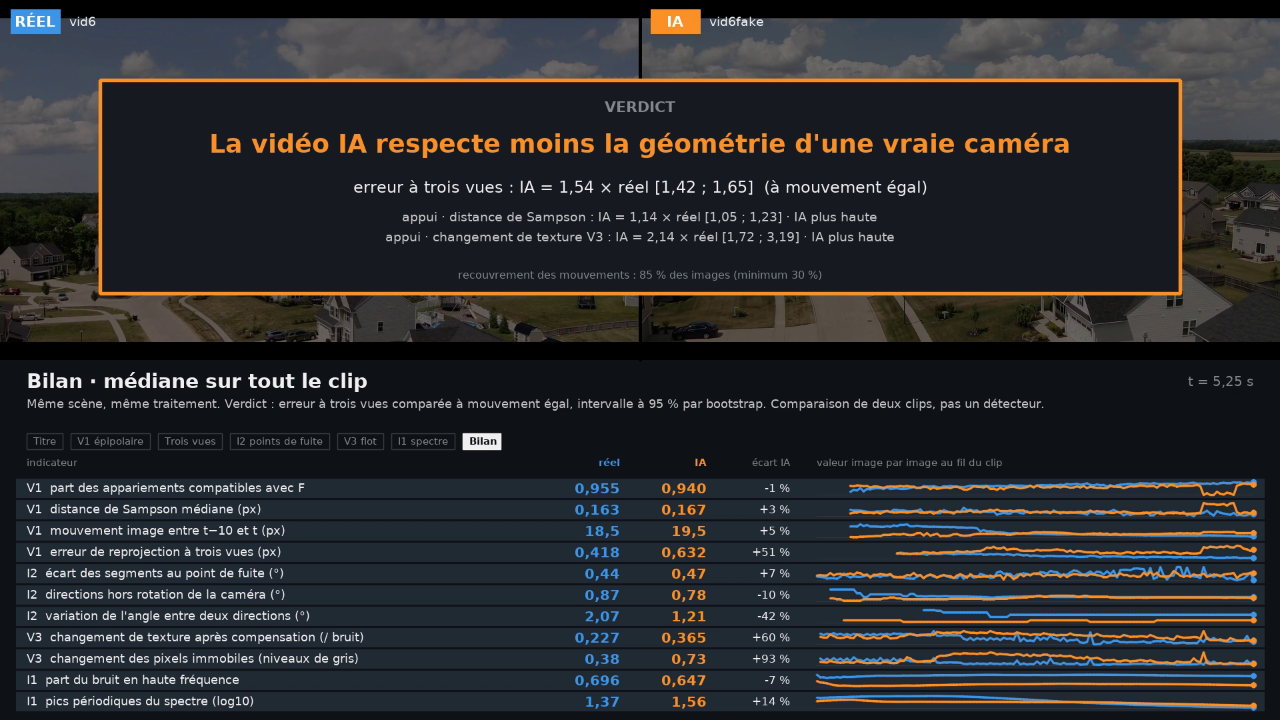
\includegraphics[width=0.8\linewidth]{demo_verdict.png}
  \caption{Last chapter of the demo on the drone scene at 1080~p: the verdict over the two
  darkened clips, then the table of medians over the clip.}
  \label{fig:verdict}
\end{figure}

% ---------------------------------------------------------------------------
\section{Discussion and limitations}

\paragraph{What the measures see.}
The controls of this project changed our conclusions more than any classifier. The raw
epipolar error, the most natural measure, mostly reflects how sharp and how stable the
rendered texture is: blur alone raises it by 41\,\%, it is as high in a copied window as in
the generated part, and its ratio changes sign across generators. The growth of the
three-view error with the frame gap removes a multiplicative change such as blur, but not an
additive noise floor nor a difference of motion; on ViF-Bench these two explain the whole
apparent effect. A geometric comparison needs equal motion \emph{and} equal precision, which is
what the comparison at equal motion of the demo does on one pair, and what a pooled benchmark
statistic does not do by itself.

\paragraph{Generators are better at geometry than we expected.}
On simple forward motion, the generators we tried keep a scene that is as rigid as the real
one at the precision of SIFT points (a fraction of a pixel at 720~p), and the two-view
constraint is almost always satisfied (the median inlier share of $F$ is within 4\,\% of the
real clip on the pairs \texttt{vid5} to \texttt{vid10}). Differences appear on some of our
scenes with large viewpoint changes (the drone
scene, where the three-view test, I2 and V5 agree), but not on ViF-Bench once motion and noise
floor are accounted for. The measures are comparative: on the drone scene the generated clip
is less rigid than its real twin, but both are within the range of real clips. Without a
matched real clip, our features are a weak detector.

\paragraph{Limits of the methods.}
V1 and the three-view test need a moving camera and a mostly static scene: people, vehicles
or wind break the single-$F$ model in real clips too, and a fixed camera gives a degenerate
case. I2 needs straight man-made structures and assumes a focal length. V5 assumes a focal
length too, relies on a learned depth that can be wrong on generated content, and reacts to
every moving object. V3 is sensitive to compression. I1 is weak on recompressed benchmarks.
The demo computes its frames offline; it is not real time. Its verdict uses one measure fixed
in advance and has only been run on six pairs.

\paragraph{What we did not do.}
A full SfM reconstruction with COLMAP (V2), image-based rendering of held-out frames (V4),
camera traces (I3) and the localization of generated regions by graph cut (I4) are not
implemented. The robustness experiment on the full ViF-Bench (re-encoding at CRF~28 and 35,
half resolution) is implemented (\texttt{src/eval/robustness.py}) but has only been run on a
12-video test subset, which is too small to report; the full run requires the school machine.
I2 and V5 have not been run on the full benchmark (V5 was stopped after 153 of 732 videos of a
40-scene subset for lack of memory), so they have no benchmark result. The selection and
weighting of the measures for the verdict on ViF-Bench, with a blind test on our pairs, is
not done yet.

% ---------------------------------------------------------------------------
\section{Conclusion}

We applied the methods of the course, from RANSAC and the normalized 8-point algorithm to the
triangulation and camera DLT of the Structure-from-Motion lecture, vanishing points, optical
flow and Fourier analysis, to measure whether generated videos respect the physics of a
camera. With careful controls, the measures separate what comes from rendering from what
comes from 3D geometry, and they corrected two of our own first readings: the raw epipolar
gap was rendering, and the higher growth of the three-view error on ViF-Bench was motion and
noise floor. Generators keep a rigid scene on simple camera paths; on some of our scenes with
large viewpoint changes the generated clip is less rigid than its real twin, and the
three-view test, the vanishing directions and the rigid-flow test (V5, outside the course)
agree there. As a detector our interpretable features reach an AUC of 0.65, below a CLIP linear
probe (0.77) but equal to it on image-to-video generators, and a late fusion with CLIP adds
$+0.018$. The natural next steps are a static-scene benchmark with large viewpoint changes,
I2 and V5 on the full benchmark, the choice of the verdict measures on ViF-Bench with a blind
test on our pairs, COLMAP reconstructions, and the robustness study on the full benchmark.

\paragraph{Code and reproducibility.}
All code, configuration files and instructions are in the repository
(\url{https://github.com/khalilzzz/CVprojet}, see \texttt{README.txt}). Seeds are fixed, every
parameter is in \texttt{configs/}, and every number in this report comes from
\texttt{results/} produced by \texttt{python -m src.run}, \texttt{python -m src.eval.inspect\_video}
and \texttt{demo.py}.

% TODO: work split between the two members
% \paragraph{Work split.} ...

\bibliographystyle{plainnat}
\bibliography{references}

\end{document}
